\section{Tiny Tapeout 4}
\label{sec:tinytapeout4}

The biggest limitations of the scan chain based architecture used in Tiny Tapeout 1 through 3 inclusive were its limited IO bandwidth and high latency.
It was decided that a new architecture was needed for Tiny Tapeout 4 and proposals were gathered from the community.
An online video call was held with community members, and the ten submitted architecture proposals discussed.

The winning architecture was a straightforward multiplexer design, shown in Fig.~\ref{fig:multiplexer_design}. This architecture was chosen as the simplest to implement while providing the most benefit in terms of additional IOs and higher bandwidth.

\begin{figure}[!t]
\centering
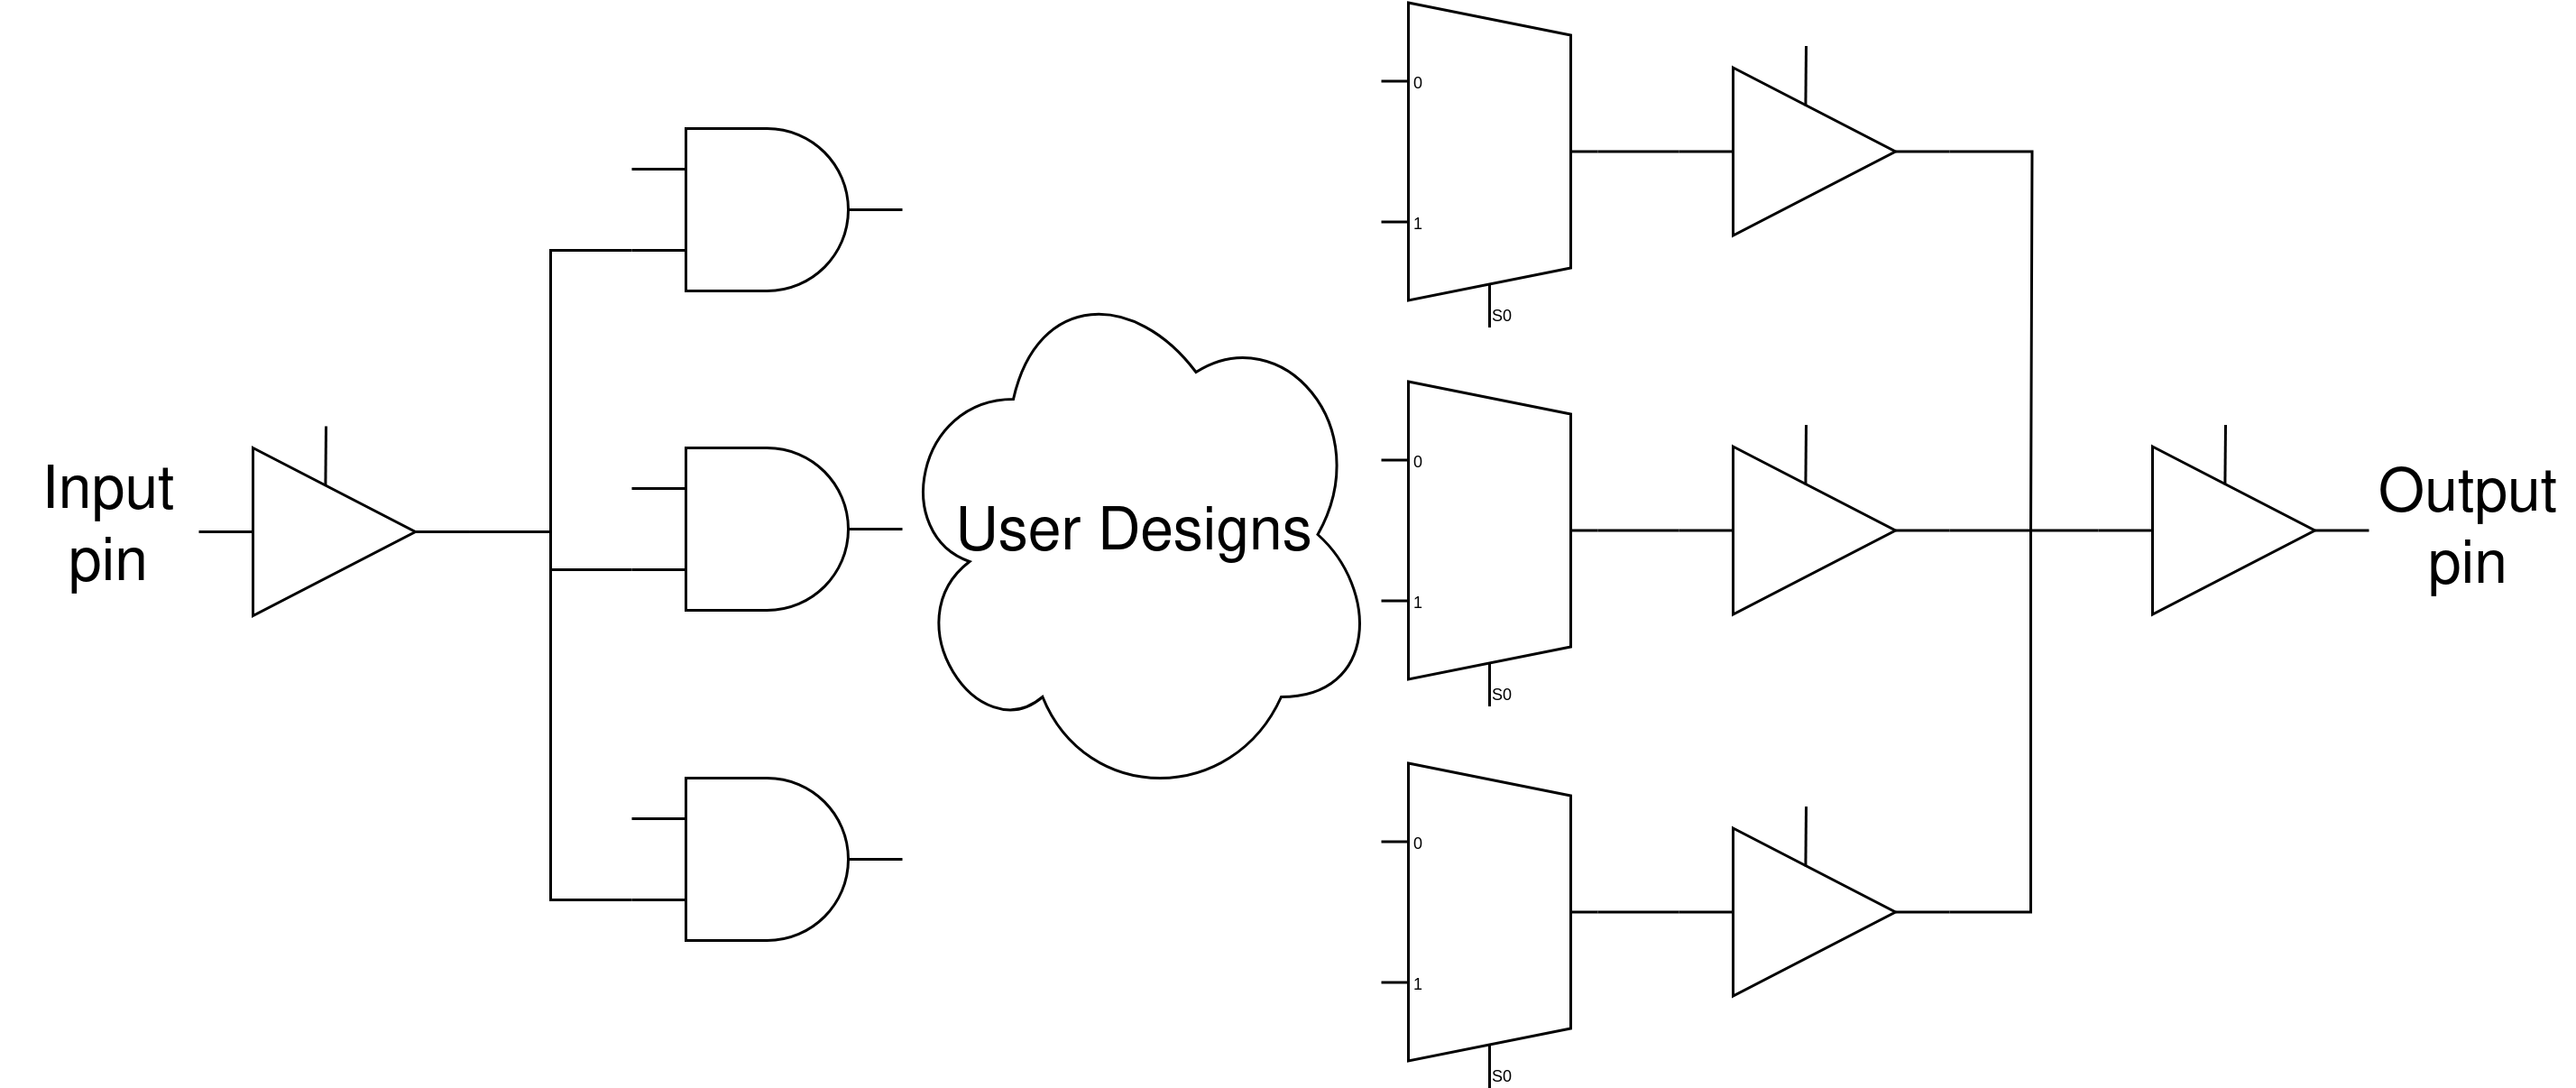
\includegraphics[width=\columnwidth]{./Figs/mux architecture.png}
\caption{A simplified diagram of the Tiny Tapeout 4 multiplexer architecture.}
\label{fig:multiplexer_design}
\end{figure}

The physical layout tested in Tiny Tapeout 3.5 and finalized in Tiny Tapeout 4 (shown in Fig.~\ref{fig:TT03_5_test_design}) consists of a central controller connected up and down to two vertical wiring spines.
For this experimental run we also included loopback test designs at the end of each multiplexer so we could measure performance for each multiplexer position.

Twenty-four horizontal multiplexers connect to the wiring spines, each of which supports 16 designs.
This allows for up to 384 separate single tile designs.
The new architecture also enabled multiple tile designs, allowing a maximum project size of $8 \times 2$ tiles or $1359 \times \qty{225}{\um\squared}$---around \num{20000} logic cells. Table~\ref{tab:comparison_TT03_TT04} shows the key differences between Tiny Tapeout 3 and Tiny Tapeout 4.

\begin{figure}[!t]
\centering
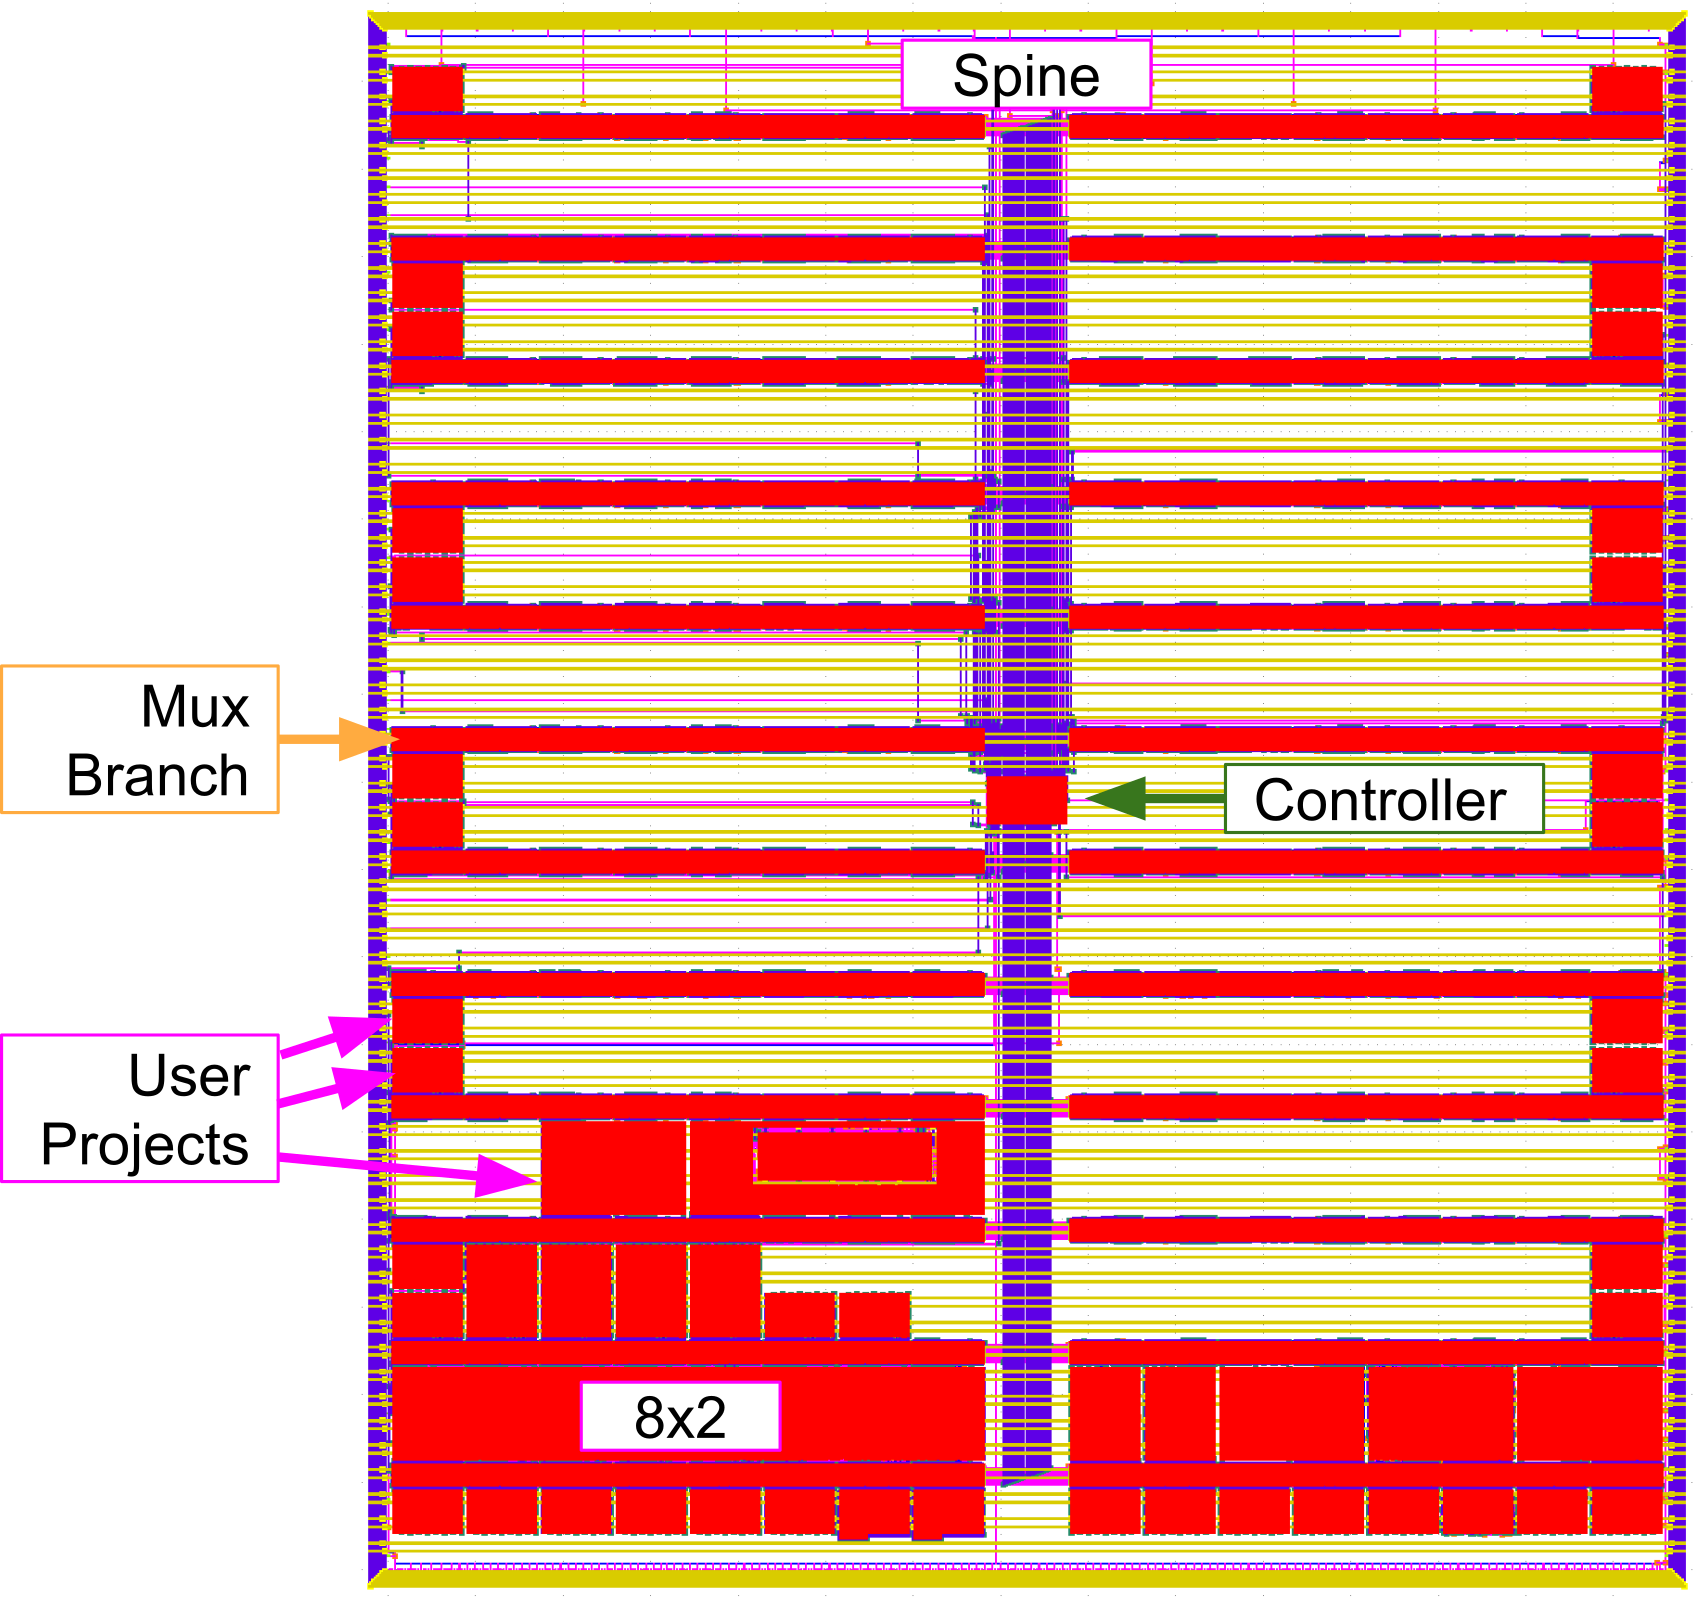
\includegraphics[width=\columnwidth]{./Figs/tt3p5 layout.png}
\caption{The Tiny Tapeout 3.5 test design.}
\label{fig:TT03_5_test_design}
\end{figure}

Another major limitation of the scan chain architecture used in Tiny Tapeout 1 through Tiny Tapeout 3 was the small number of IO pins.
The scan controller used nine GPIOs to select the currently active design. While this simplified the demonstration board board, it also wasted valuable IO pins.

Starting with Tiny Tapeout 4 the parallel design selection architecture used in previous chips was dropped in favor of a serial protocol.
The extra pins thus provided were then used bidirectionally, giving each design a clock pin, reset pin, and 24 IO pins.

\begin{table}[!t]
\centering
\caption{A comparison between Tiny Tapeout 3 and Tiny Tapeout 4.}
\label{tab:comparison_TT03_TT04}
\begin{tabular}{@{}lcc@{}}
\toprule
Parameters & TT03 & TT04 \\
\midrule
Max clock speed & \qty{8}{\kHz} & \qty{50}{\MHz} \\
Max design size & $150 \times \qty{170}{\um\squared}$ & $1359 \times \qty{225}{\um\squared}$ \\
Input pins & 8 & 10 \\
Output pins & 8 & 8 \\
Bidirectional IO pins & None & 8 \\
Custom GDS file & \xmark & \checkmark \\
\bottomrule
\end{tabular}
\end{table}
